\section{Interférence à double fente dans \(T^2_{27}\) : mémoire de chemin, règle de Born et unitarité dodécaphasique}
\label{sec:md-sucesora-interferometria-t27}

La réalisation finie se construit sur
\[
 \mathcal H_{\mathrm{cam}}
 =\ell^2\!\left(T_{27}^{2}\right)\otimes\mathbb C^4,
 \qquad
 T_{27}^{2}=(\mathbb Z/27\mathbb Z)^2,
\]
où le facteur de dimension \(4\) enregistre les directions
\((N,S,E,W)\). La mémoire explicite de la trajectoire ajoute le facteur
\(\mathbb C^2_{\mathrm{mem}}\). Le pas microscopique est l'opérateur
\begin{equation}
 U_{\mathrm{micro}}=S D_J C_4,
 \label{eq:md-sucesora-interferometro-microstep}
\end{equation}
avec \(C_4\) unitaire, \(D_J\) diagonal et \(S\) comme déplacement conditionné
par la direction. En conséquence,
\[
 U_{\mathrm{micro}}^*U_{\mathrm{micro}}=I,
\]
et la norme est conservée à chaque pas.

\subsection{Préparation des \(2\) trajectoires et écran de lecture}

Les deux ouvertures sont fixées en
\[
 (x_0,y_1)=(2,8),
 \qquad
 (x_0,y_2)=(2,18),
\]
avec le même état directionnel initial. Si \(\psi_1\) et \(\psi_2\) sont les
amplitudes propagées depuis chaque ouverture, l'écran situé en \(x=24\)
publie, pour un recouvrement réel de mémoire \(\mu\in[0,1]\),
\begin{equation}
 I_\mu(y)
 =\frac12\sum_d
 \left(
  |\psi_1(24,y,d)|^2+|\psi_2(24,y,d)|^2
  +2\operatorname{Re}\!\left[
   \mu\,\overline{\psi_1(24,y,d)}\psi_2(24,y,d)
  \right]
 \right).
 \label{eq:md-sucesora-interferometro-intensidad}
\end{equation}
La formule s'obtient aussi en introduisant les marqueurs
\[
 |m_1\rangle=(1,0),
 \qquad
 |m_2\rangle=(\mu,\sqrt{1-\mu^2})
\]
et en prenant la trace sur \(\mathbb C^2_{\mathrm{mem}}\). Cette égalité identifie le
recouvrement des registres, non une perte de norme, comme origine de
l'atténuation des franges. En particulier,
\begin{equation}
 \mathcal V(\mu)=|\mu|\,\mathcal V(1).
 \label{eq:md-sucesora-interferometro-visibilidad}
\end{equation}
Pour \(\mu=0\), une correction de phase ne peut pas reconstruire le terme croisé ;
si les marqueurs sont défaits unitairement avant la recombinaison, on
retrouve exactement la courbe \(\mu=1\).

\subsection{Identités d'unitarité de l'ordre dodécaphasique sous un budget commun d'amplitude}

Le bloc de contrôle comporte \(12\) impulsions orientées et une somme vectorielle nulle.
Les \(6\) premières sont obtenues à partir d'un germe directionnel au moyen de la signature
dodécaphasique ; les \(6\) restantes sont leurs opposées. On compare quatre
séquences de \(36\) pas :
\begin{enumerate}
 \item la séquence canonique, répétée pendant \(3\) cycles complets ;
 \item son inversion orientée ;
 \item une séquence dans laquelle une paire opposée est remplacée par des phases communes
       de même norme ;
 \item une permutation aléatoire du même multiensemble d'impulsions.
\end{enumerate}
Toutes conservent le nombre d'impulsions, la somme vectorielle nulle et le budget
quadratique. La différence entre leurs motifs mesure donc la dépendance
à l'ordre non commutatif et à l'information directionnelle, non une
injection inégale de norme ou d'énergie.

La non-commutativité se vérifie sur un état sonde fixé avant la
lecture :
\[
 \left\|U_bU_a\psi-U_aU_b\psi\right\|_2
 =0.24776388825652637.
\]
Le contrôle numérique fournit
\[
 \|C_4^*C_4-I\|_{\max}=0,
 \qquad
 \max_t\bigl|\|\psi_t\|_2^2-1\bigr|
 =1.3322676295501878\times10^{-15},
\]
\[
 \Delta B_2=2.220446049250313\times10^{-16},
 \qquad
 \varepsilon_{\mathrm{Born}}
 =1.734723475976807\times10^{-18},
\]
\[
 \varepsilon_{\mathcal V(\mu)}
 =2.220446049250313\times10^{-16},
\]
où \(\Delta B_2\) est la dispersion maximale du budget quadratique entre
les quatre séquences.

\begin{table}[tbp]
\centering
\caption{Interférence et distance par rapport à la séquence canonique après \(36\) pas.}
\label{tab:md-sucesora-interferometro-resultados}
\begin{tabular}{lccc}
\toprule
Séquence & \(\mathcal V_{\mathrm{lineal}}\) &
distance de variation totale & fidélité moyenne \\
\midrule
canonique      & \(0.5992212256\) & \(0\)            & \(1.0000000000\) \\
inverse       & \(0.5974219552\) & \(0.0333923142\) & \(0.9740951119\) \\
paire remplacée& \(0.5907431085\) & \(0.0628288605\) & \(0.9417893564\) \\
randomisée  & \(0.6254301808\) & \(0.0963185652\) & \(0.6564185376\) \\
\bottomrule
\end{tabular}
\end{table}

\subsection{Interférence reconstruite dans \(T^2_{27}\) : distribution de détection et domaine physique}

\begin{theorem}[Interférence unitaire avec mémoire explicite de chemin]
Pour la dynamique définie par \eqref{eq:md-sucesora-interferometro-microstep},
l'intensité obtenue en prenant la trace sur le registre de chemin coïncide avec
\eqref{eq:md-sucesora-interferometro-intensidad} ; la visibilité satisfait
\eqref{eq:md-sucesora-interferometro-visibilidad} ; et des séquences ayant un budget
quadratique identique peuvent produire des motifs distincts lorsque leur
ordre diffère.
\end{theorem}

La démonstration est finie : unitarité de chaque facteur, développement du carré
de la somme des deux branches et contraction partielle du marqueur. Les contrôles
numériques précédents vérifient l'exécution sur \(T_{27}^{2}\). La carte
concrète qui envoie l'état dodécaphasique sur des phases directionnelles constitue une
réalisation physique déclarée ; elle n'est pas identifiée par définition au retour
temporel de \(108\) phases. L'échelle électronique est appliquée après la
dynamique adimensionnelle et ne sélectionne pas le mot ni n'ajuste les franges.

La réalisation serait réfutée par une perte d'unitarité, une divergence entre
la mémoire explicite et la règle de Born, la création d'interférence par une phase
lorsque \(\mu=0\), la dépendance du budget énergétique entre séquences ou l'utilisation
du résultat de l'écran pour choisir rétrospectivement l'ordre des
impulsions.

\begin{figure}[tbp]
\centering
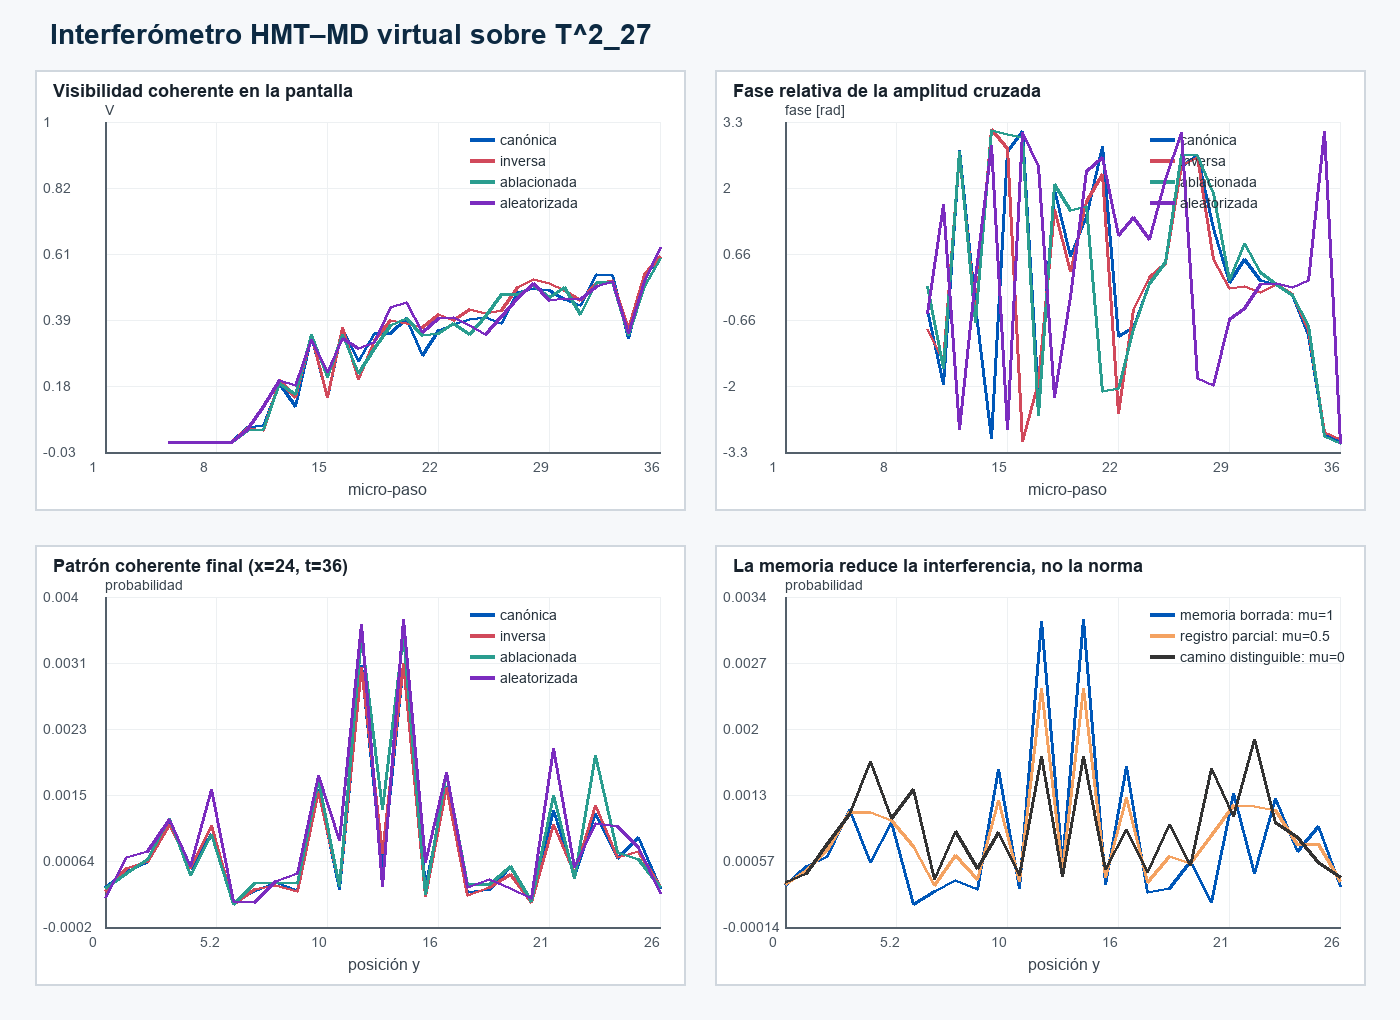
\includegraphics[width=.96\linewidth]{figures/parte_iv/01_curvas_y_patrones.png}
\caption[Évolution de la visibilité, de la phase relative et du motif final pour les quatre séquences à budget commun.]{Évolution de la visibilité, de la phase relative et du motif final pour les quatre séquences à budget commun. \textit{Traduction des libellés de l'image :} « Interféromètre virtuel HMT--MD sur \(T^2_{27}\) ». Panneaux : visibilité cohérente sur l'écran ; phase relative de l'amplitude croisée ; motif cohérent final (\(x=24\), \(t=36\)) ; la mémoire réduit l'interférence, non la norme. Axes : micro-pas, position \(y\), phase [rad], probabilité. Séries : canonique, inverse, avec ablation, aléatoire ; mémoire effacée (\(\mu=1\)), enregistrement partiel (\(\mu=0{,}5\)), chemin discernable (\(\mu=0\)).}
\label{fig:md-sucesora-interferometro-patrones}
\end{figure}

\begin{figure}[tbp]
\centering
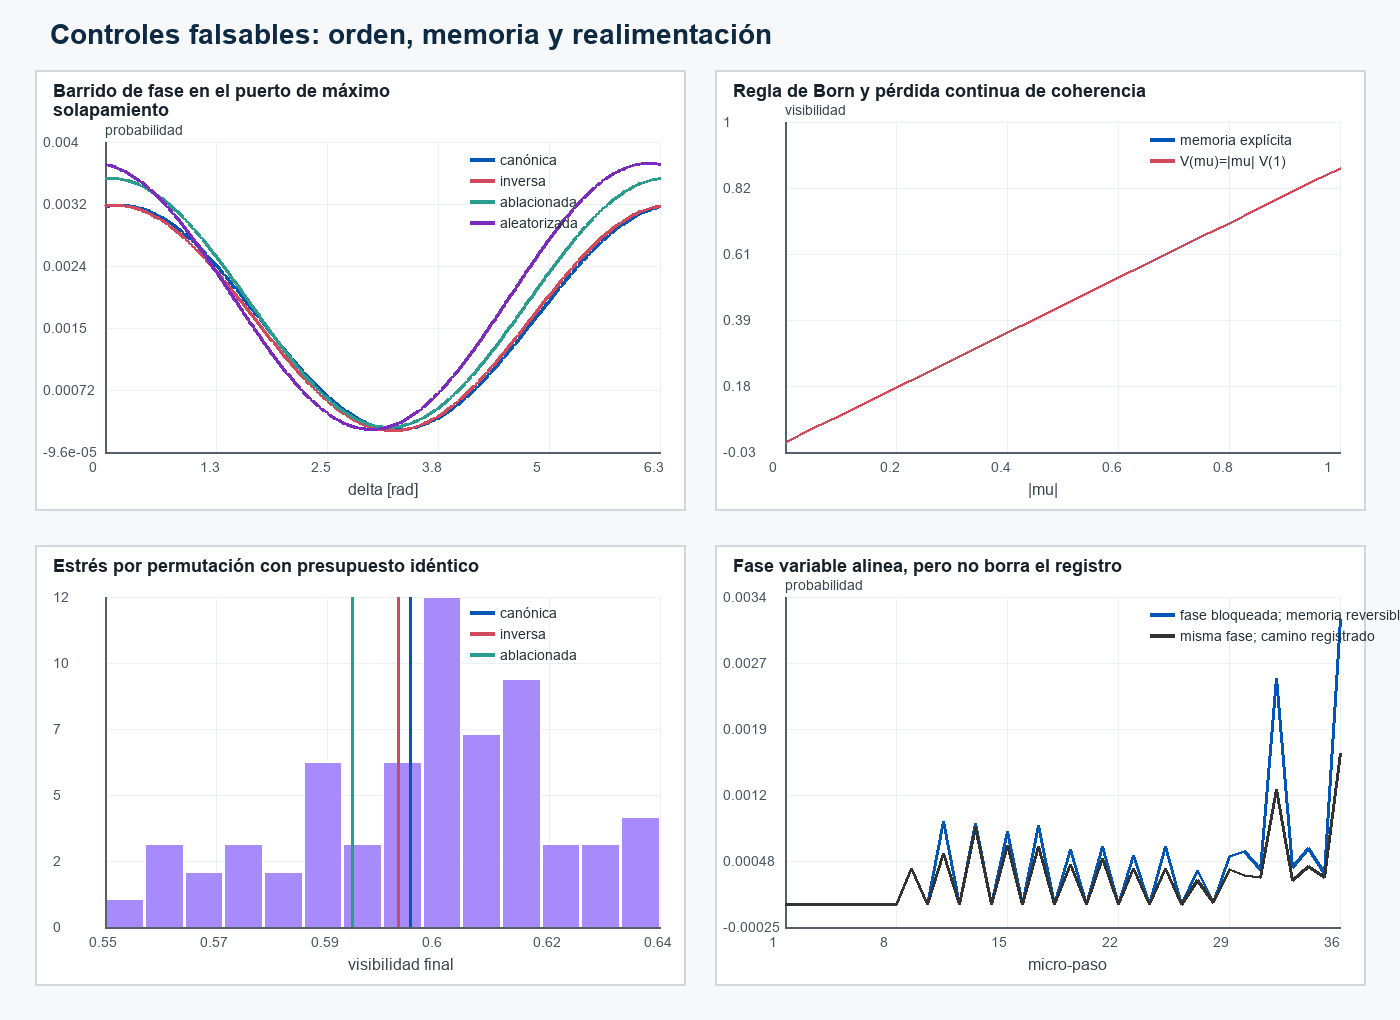
\includegraphics[width=.96\linewidth]{figures/parte_iv/02_estres_memoria_y_control.png}
\caption[Contrôles de l'ordre, de la mémoire de chemin et de la rétroaction de phase.]{Contrôles de l'ordre, de la mémoire de chemin et de la rétroaction de phase. \textit{Traduction des libellés de l'image :} « Contrôles falsifiables d'ordre, de mémoire et de rétroaction ». Panneaux : balayage de phase au port de recouvrement maximal ; règle de Born et perte continue de cohérence ; permutations à budget identique ; la phase variable aligne, mais n'efface pas l'enregistrement. Axes : probabilité, visibilité, \(\delta\) [rad], \(\lvert\mu\rvert\), visibilité finale, micro-pas. Séries : canonique, inverse, avec ablation, aléatoire ; mémoire explicite ; phase verrouillée, mémoire réversible ; même phase, chemin enregistré.}
\label{fig:md-sucesora-interferometro-controles}
\end{figure}
